\section{Worker-Node Execution Pipeline (\texttt{nodescript.\allowbreak{}sh} / \texttt{functions.\allowbreak{}sh})}\label{ch:9}

\subsection{Self-documenting nodescript convention}

Every pipeline step in the generated \texttt{nodescript.\allowbreak{}sh} follows the same four-part pattern: a \texttt{\# input:\allowbreak{} \ldots{} output:\allowbreak{} \ldots{}} comment, an explicit \texttt{cmd=\allowbreak{}(.\allowbreak{}.\allowbreak{}.\allowbreak{})} bash array holding the full invocation, a descriptive \texttt{echo "Running <Step>:\allowbreak{} \$\{cmd[@]\}"}, and \texttt{run\_\allowbreak{}timed <fn> "\$\{cmd[@]\}"} which times the step and forwards the command to a thin wrapper in \texttt{functions.\allowbreak{}sh}. The wrappers add error handling and cleanup (removing intermediate files, \texttt{df} checks) but construct no commands. The result is a script a user can read top-to-bottom and re-run verbatim.

\subsection{Preamble}

\texttt{create\_\allowbreak{}preamble.\allowbreak{}py} emits the shebang, argument parsing (\texttt{sjob} = \texttt{\$1}; for type-2, \texttt{lundFile} = \texttt{\$2} and \texttt{lund\_\allowbreak{}base} derived from it), \texttt{set -\allowbreak{}euo pipefail}, the output directory, sourcing of \texttt{functions.\allowbreak{}sh}, and the exit-code definitions.

\subsection{Environment setup}

The script sets \texttt{CLAS12\_\allowbreak{}CONFIG} (the coatjava/gemc config tree on CVMFS), \texttt{OSRELEASE=\allowbreak{}almalinux9-\allowbreak{}gcc11} so CVMFS modulefiles resolve to the platform directory containing GEMC/JDK/HIPO/denoise, the module system, and \texttt{RCDB\_\allowbreak{}CONNECTION} for run conditions.

\subsection{Module-loading strategy}

Modules are loaded and unloaded per step with pinned versions (\texttt{gemc}, \texttt{coatjava}, \texttt{mcgen} from the scard), with availability checks, so each stage runs against exactly the requested software.

\subsection{Pelican / OSDF environment}

\texttt{BEARER\_\allowbreak{}TOKEN\_\allowbreak{}FILE} (injected by the CredMon via the Condor OAuth service) authorizes all Pelican transfers on the node --- LUND fetch and output upload alike.

\subsection{Input stage}

\texttt{create\_\allowbreak{}lund\_\allowbreak{}or\_\allowbreak{}generator.\allowbreak{}py} emits one of three input paths: \textbf{type-2} fetches the assigned LUND file with \texttt{pelican object get}; an \textbf{external generator} runs the generator command array to produce events; a \textbf{GEMC-internal generator} produces events inside GEMC and needs no separate input step.

\begin{itemize}
  \item \textbf{9.6.1 Seed generation.} External generators receive a per-subjob random seed so subjobs are statistically independent.
  \item \textbf{9.6.2 Run-by-run weighted selection.} For run-dependent requests, \texttt{select\_\allowbreak{}weighted\_\allowbreak{}run} (calling \texttt{select\_\allowbreak{}run.\allowbreak{}py}) draws a run number from the staged run list weighted by luminosity/exposure, so the sample reproduces the run-mix of real data. This is the runtime half of the run-by-run feature staged in Chapter 7.7.
\end{itemize}

\subsection{GEMC execution}

\texttt{create\_\allowbreak{}run\_\allowbreak{}gemc.\allowbreak{}py} resolves the gcard for the configuration and builds the full \texttt{cmd=\allowbreak{}(gemc \ldots{})} array: the gcard, number of events, torus/solenoid scales from \texttt{fields}, vertex/z-position and raster handling, beam settings, and the output \texttt{gemc.\allowbreak{}hipo}.

\subsection{Background merging}

When \texttt{bkmerging} is set, \texttt{fetch\_\allowbreak{}background\_\allowbreak{}file} pulls a random background HIPO file from OSDF and \texttt{merge\_\allowbreak{}background} merges it into the GEMC output over the configured detector list, producing \texttt{gemc.\allowbreak{}merged.\allowbreak{}hipo} (and removing the inputs).

\subsection{Denoising}

For coatjava older than 14, \texttt{run\_\allowbreak{}denoiser} (\texttt{denoise2.\allowbreak{}exe}) runs on the merged/GEMC file. For coatjava 14 and newer the step is skipped and reconstruction reads the merged (or plain) GEMC file directly.

\subsection{Reconstruction}

\texttt{run\_\allowbreak{}reconstruction} runs \texttt{recon-\allowbreak{}util} with the YAML appropriate to the request (an \texttt{mc-\allowbreak{}ai} configuration for AI-assisted tracking, or the experiment configuration), producing \texttt{recon.\allowbreak{}hipo}.

\subsection{Integrity test}

\texttt{test\_\allowbreak{}hipo\_\allowbreak{}file} runs \texttt{hipo-\allowbreak{}utils -\allowbreak{}test} on the reconstructed file to catch truncated or corrupt output before it is promoted to a DST.

\subsection{DST creation vs. rename}

\texttt{create\_\allowbreak{}dst} reduces the reconstructed file to the DST bank list, honoring \texttt{dstOUT}, producing the final \texttt{\$OUTPUT\_\allowbreak{}FILE}. In the GEMC-only branch there is no DST step --- the GEMC output is renamed to \texttt{\$OUTPUT\_\allowbreak{}FILE}.

\subsection{Output filename convention}

\texttt{get\_\allowbreak{}output\_\allowbreak{}filename} builds \texttt{\$OUTPUT\_\allowbreak{}FILE} as \texttt{<string\_\allowbreak{}id>-\allowbreak{}<submission\_\allowbreak{}id>-\allowbreak{}<sjob>.\allowbreak{}hipo} (type-1) or \texttt{<string\_\allowbreak{}id>-\allowbreak{}<lund\_\allowbreak{}base>-\allowbreak{}<submission\_\allowbreak{}id>-\allowbreak{}<sjob>.\allowbreak{}hipo} (type-2), so every subjob's output is uniquely named and traceable back to its submission.

\subsection{Output upload}

\texttt{write\_\allowbreak{}to\_\allowbreak{}jlab} uploads \texttt{\$OUTPUT\_\allowbreak{}FILE} to the per-user OSDF volatile namespace (\texttt{osdf:\allowbreak{}/\allowbreak{}/\allowbreak{}/\allowbreak{}jlab-\allowbreak{}osdf/\allowbreak{}clas12/\allowbreak{}volatile/\allowbreak{}osg/\allowbreak{}<user>/\allowbreak{}<sub\_\allowbreak{}id>/\allowbreak{}}).

\subsection{GEMC-only branch}

For \texttt{output\_\allowbreak{}type =\allowbreak{} 1}, the pipeline stops after GEMC (and optional background merging): the GEMC file is renamed to \texttt{\$OUTPUT\_\allowbreak{}FILE} and uploaded directly, skipping denoising, reconstruction, integrity test, and DST.

\subsection{Timing instrumentation}

\texttt{run\_\allowbreak{}timed} records each step's wall time in a timing registry, and \texttt{print\_\allowbreak{}timing\_\allowbreak{}summary} emits a per-step breakdown at the end of the job --- the basis for the timing figures and for spotting a slow stage.

\subsection{Exit-code taxonomy}

Each step maps failures to specific exit codes; the transient subset (Chapter 8.3) is exactly the set \texttt{periodic\_\allowbreak{}release} retries. This coupling --- the nodescript's exit codes and the Condor card's release policy --- is what turns transient OSG failures into automatic retries and real bugs into held jobs. The full catalogue is in Appendix E.

\subsection{The complete file chain}

\begin{figure}[htbp]
  \centering
  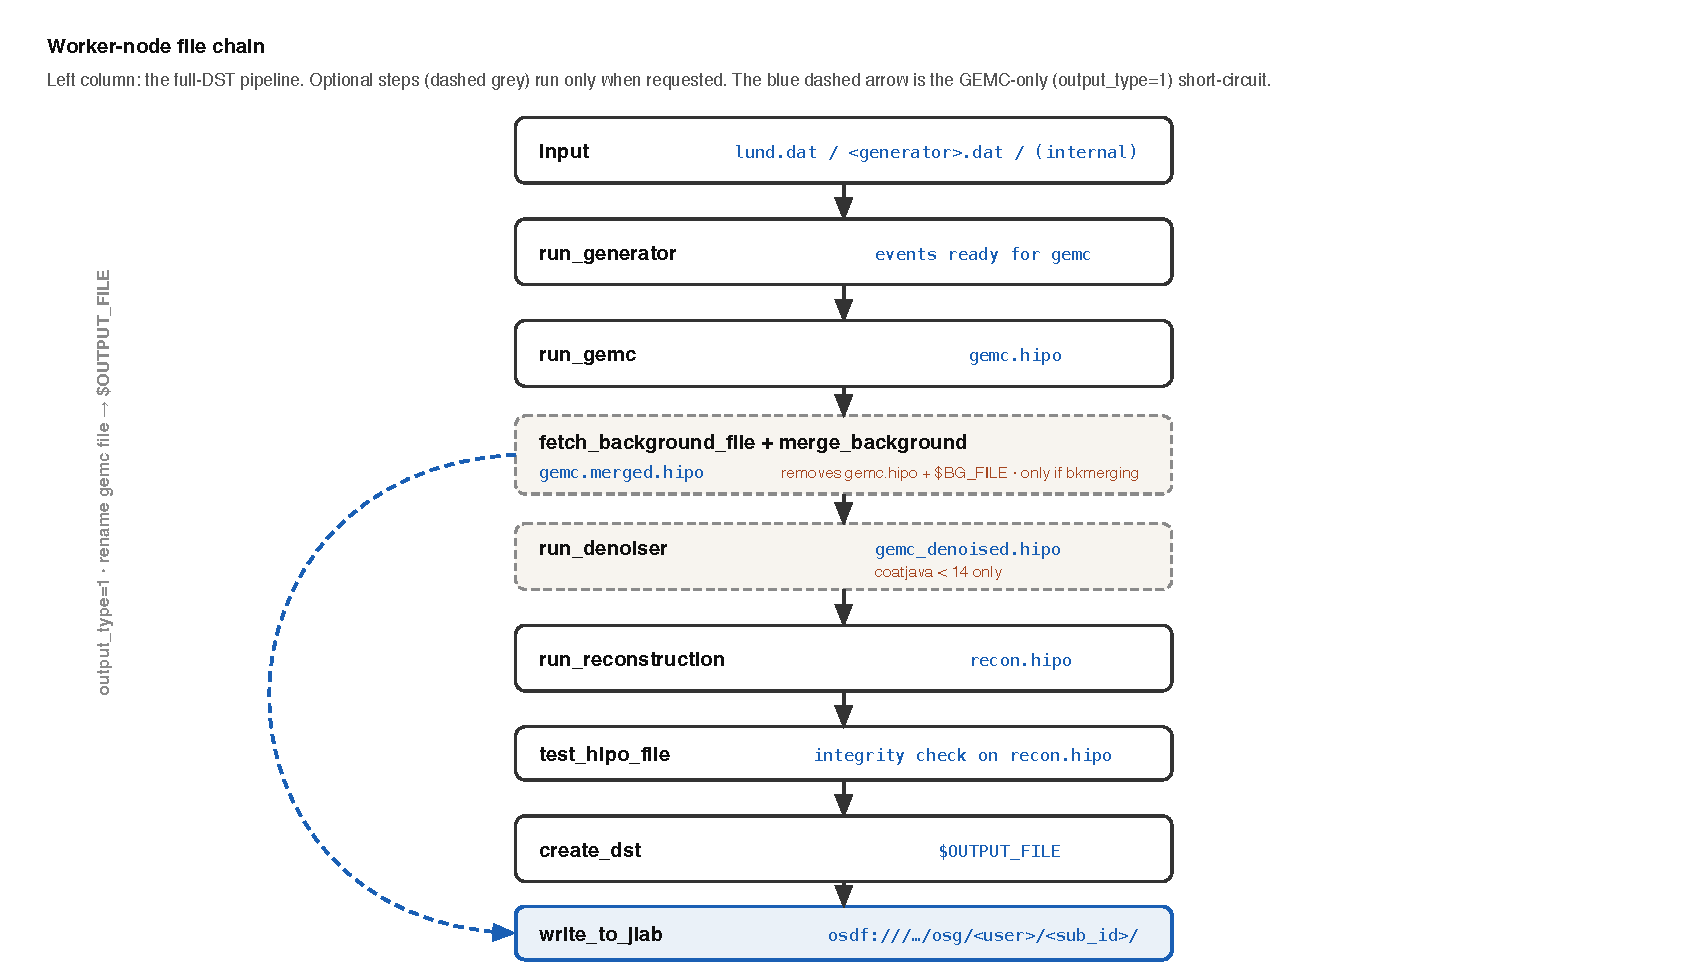
\includegraphics[width=0.8\textwidth]{figures/fig3_file_chain}
  \caption{Worker-node file chain. Left column: the full-DST pipeline. Optional steps run only when requested; the dashed arrow is the GEMC-only (\texttt{output\_type=1}) short-circuit that renames the GEMC output and uploads it directly.}
  \label{fig:filechain}
\end{figure}
